\chapter{Relación Agua, Suelo, Planta, Atmósfera}
\subsubsection{Factores a tomar en cuneta}
\begin{enumerate}
    \item La composición química de ésta
    \item La tolerancia de los cultivos a las sales
    \item Las propiedades físicas y químicas de los suelos
    \item Las prácticas de manejo de suelos, aguas y cultivos
    \item Las condiciones climatológicas
    \item El método de riego por emplear
    \item Las condiciones de drenaje interno y superficial del suelo
\end{enumerate}

La metodología del USDA (laboratorio de Riverside), esta metodología toma en consideración dos índices:
\begin{itemize}
    \item Conductividad eléctrica (CE)
    \item Relación de adsorción de sodio
\end{itemize}
El rango de validez: $3<CE\times 10^3<30$
\begin{equation}
    PO = 0.36(CE\times 10^3)
\end{equation}
% Generalmente se expresa en desimenes
El rango de validez: $100<CE\times 10^6<5000$
\begin{equation}
    PPM = 0.64(CE\times 10^6)
\end{equation}
Rango de validez: $0.1<CE\times 10^3<5$
\begin{equation}
    \frac{me}{L} = 10(CE\times 10^3)
\end{equation}
\subsubsection{Relación de adsorción de sodio (RAS)}
\begin{figure}[h!]
\centering
  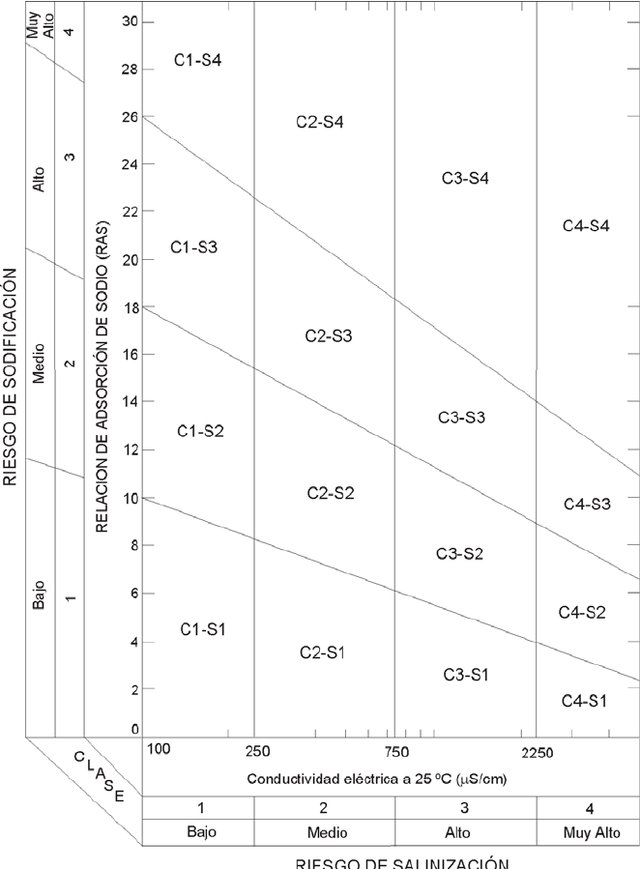
\includegraphics[width=0.5\textwidth]{raspa1.jpg}
  \caption{Clasificación de aguas de riego, según USDA (1956)\cite{keller1956results}}
  \label{raspa1}
\end{figure}
La RAS se calcula con la siguiente ecuación:
\begin{equation}
    RAS = \frac{NA}{\sqrt{\frac{Ca + Mg}{2}}}
\end{equation}
En la que los valores de Na, Ca y Mg están dados en $me/l$ y los valores del RAS en $(me/l)^{1/2}$. Cuando se aplica sodio en exceso a un suelo, através del agua de riego, se destruye la estructura del mismo, conociéndose esto como defloculación. La RAS, se clasifica en base a la figura en $S_1$, $S_2$, $S_3$ y $S_4$
\begin{table}[h!]
    \centering
    \begin{tabular}{lll}
    Criterios &
      Índices &
      Símbolos \\
    Contenido de sales solubles &
      \begin{tabular}[c]{@{}l@{}}Conductividad eléctrica\\ Salinidad efectiva\\ Salinidad potencial\end{tabular} &
      \begin{tabular}[c]{@{}l@{}}CE\\ SE\\ SP\end{tabular} \\
    \begin{tabular}[c]{@{}l@{}}Efecto probable del \\ sodio sobre las \\ características físicas\\ del suelo\end{tabular} &
      \begin{tabular}[c]{@{}l@{}}Relación de adsorción del sodio\\ Carbonato de sodio residual\end{tabular} &
      \begin{tabular}[c]{@{}l@{}}RAS\\ CSR\end{tabular} \\
    \begin{tabular}[c]{@{}l@{}}Contenido de elementos\\ tóxicos para las plantas\end{tabular} &
      \begin{tabular}[c]{@{}l@{}}Contenido de boro\\ Contenido de cloruros\end{tabular} &
      \begin{tabular}[c]{@{}l@{}}B\\ Cl\end{tabular}
    \end{tabular}
    \caption{Metodología de Palacios y Aceves (1970)\cite{palacios1970instructivo}}
    \label{tabraspa1}
\end{table}
De la salinidad efectiva (SE), se calcula con algunas de las siguientes fórmulas y bajo las condiciones:
\begin{itemize}
    \item Si $Ca> (CO_3+HCO_3+SO_4)$, entonces $SE=$ suma de cationes-$(CO_3+HCO_3+SO_4)$
    \item Si $Ca<(CO_3+HCO_3+SO_4)$, pero $Ca> (CO_3+HCO_3)$ entonces $SE=$ suma de cationes - $Ca$
\end{itemize}
% INCOMPLETO
\subsubsection{Efecto probable del sodio sobre las características físicas del suelo}
Relación de adsorción de sodio (RAS) y carbonato de sodio residual (CSR):
\begin{equation}
    CSR = (CO_3 + HCO_3) -(Ca + Mg)
\end{equation}
\begin{table}[h!]
    \centering
    \begin{tabular}{@{}cccc@{}}
    \toprule
    \multirow{2}{*}{Cultivo} & \multicolumn{3}{c}{Disminución del Rend} \\ \cmidrule(l){2-4} 
                             & 100          & 250         & 500         \\ \cmidrule(r){1-1}
    Cultivos comunes         & \multicolumn{3}{c}{Ce (mmhos)}           \\
    Cebada                   & 120          & 160         & 180         \\
    Remolacha                & 100          & 110         & 100         \\
    Algodonero               & 100          & 120         & 180         \\
    Centeno                  & 100          & -           & 100         \\
    Cártamo                  & 77           & 110         & 140         \\
    Trigo                    & 70           & 110         & 140         \\
    Sorgo                    & 60           & 90          & 120         \\
    Soya                     & 60           & 70          & 90          \\
    Arroz                    & 50           & 50          & 80          \\
    Maíz                     & 60           & 80          & 70          \\
    Avena                    & 40           & 90          & 100         \\
    Sesbania                 & 40           & 80          & 90          \\
    Haba                     & 40           & 50          & 70          \\
    Linaza                   & 30           & 50          & 70          \\
    Frijol                   & 10           & 20          & 30          \\ \bottomrule
    \end{tabular}
    \caption{Tolerancia de los cultivos a la salinidad del extracto de saturación del suelo}
    \label{tabraspa2}
\end{table}
\begin{table}[h!]
    \centering
    \begin{tabular}{@{}|c|c|ccc|@{}}
    \toprule
    \multirow{2}{*}{Problema potencial} &
      \multirow{2}{*}{Unidades} &
      \multicolumn{3}{c|}{Grados de restricción de uso} \\ \cmidrule(l){3-5} 
     &
       &
      \multicolumn{1}{c|}{Ningúna} &
      \multicolumn{1}{c|}{\begin{tabular}[c]{@{}c@{}}Ligera a\\ moderada\end{tabular}} &
      Severo \\ \midrule
    \begin{tabular}[c]{@{}c@{}}Salinidad (afecta disponibilidad de agua\\ para el culivo)\\ ECa o\\ Tss\end{tabular} &
      \begin{tabular}[c]{@{}c@{}}dS/mol\\ mg/L\end{tabular} &
      \multicolumn{1}{c|}{\begin{tabular}[c]{@{}c@{}}<0.7\\ <450\end{tabular}} &
      \multicolumn{1}{c|}{\begin{tabular}[c]{@{}c@{}}0.7-3.0\\ 450-2000\end{tabular}} &
      \begin{tabular}[c]{@{}c@{}}>30\\ <2000\end{tabular} \\ \midrule
    \begin{tabular}[c]{@{}c@{}}Infiltración (reduce infiltración; evaluar\\ usando a la vez la ECa y el RAS)\\ Ras=0-3 y Eca=\\ =3.6 y Eca=\\ =6-12 y Eca=\\ =12-20 y Eca=\\ =20-04 y Eca\end{tabular} &
       &
      \multicolumn{1}{c|}{\begin{tabular}[c]{@{}c@{}}>0.7\\ >1.2\\ >1.9\\ >2.9\\ >5.0\end{tabular}} &
      \multicolumn{1}{c|}{\begin{tabular}[c]{@{}c@{}}0.7-0.2\\ 1.2-0.3\\ 1.9-0.5\\ 2.9-1.3\\ 5.0-2.9\end{tabular}} &
      \begin{tabular}[c]{@{}c@{}}<0.2\\ <0.3\\ <0.5\\ <1.3\\ <2.9\end{tabular} \\ \midrule
    \begin{tabular}[c]{@{}c@{}}Toxicidad de iones específicos\\ (cultivos sensibles)\\ Sodio $(Na)^+$\\ Riego por superficie\\ Riego por aspersión\\ Cloro $(Cl))^+$\\ Riego por superficie\\ Riego por aspersión\\ Boro (B)\\ Oligoelementos\end{tabular} &
      \begin{tabular}[c]{@{}c@{}}RAS\\ me/L\\ \\ me/L\\ me/L\\ me/L\end{tabular} &
      \multicolumn{1}{c|}{\begin{tabular}[c]{@{}c@{}}<3\\ <3\\ \\ <4\\ <3\\ <0.7\end{tabular}} &
      \multicolumn{1}{c|}{\begin{tabular}[c]{@{}c@{}}3.9\\ >3\\ \\ 4.0-10\\ >3\\ 0.7-3.0\end{tabular}} &
      \begin{tabular}[c]{@{}c@{}}>9\\ \\ \\ >10\\ \\ >30\end{tabular} \\ \midrule
    \begin{tabular}[c]{@{}c@{}}Varios (afecta cultivos sensibles)\\ Nitrogeno $(NO_3-N)$\\ Bicarbonato $(HCO_3-N)$\\ (Aspersión foliar únicamente) \\ pH\end{tabular} &
      \begin{tabular}[c]{@{}c@{}}mg/L\\ \\ mg/L\end{tabular} &
      \multicolumn{1}{c|}{\begin{tabular}[c]{@{}c@{}}<5\\ \\ <1.5\\ amplitud\end{tabular}} &
      \multicolumn{1}{c|}{\begin{tabular}[c]{@{}c@{}}5.03-30\\ \\ 1.5-8.5\\ Normal: 6.5-8.4\end{tabular}} &
      \begin{tabular}[c]{@{}c@{}}>30\\ \\ >8.5\end{tabular} \\ \bottomrule
    \end{tabular}
    \caption{Tolerancia de los cultivos a la salinidad del extracto de saturación del suelo, etc.}
    \label{tabraspa3}
\end{table}
\subsection{Propiedades Físicas del Suelo}
Es aquella cualidad distintiva que se basa principalmente en la composición física del suelo, que puede ser visible y medible y que no varía con el tiempo
\begin{itemize}
    \item Textura
    \item Color
    \item Densidad Real
\end{itemize}
\subsubsection{Textura del Suelo}
Se refiere a la proporción de arenas, limo y arcilla, para determinarla existen diferentes métodos como la estimación al tacto, método de la pipeta y el método de Bouyoucos
\begin{figure}[h!]
\centering
  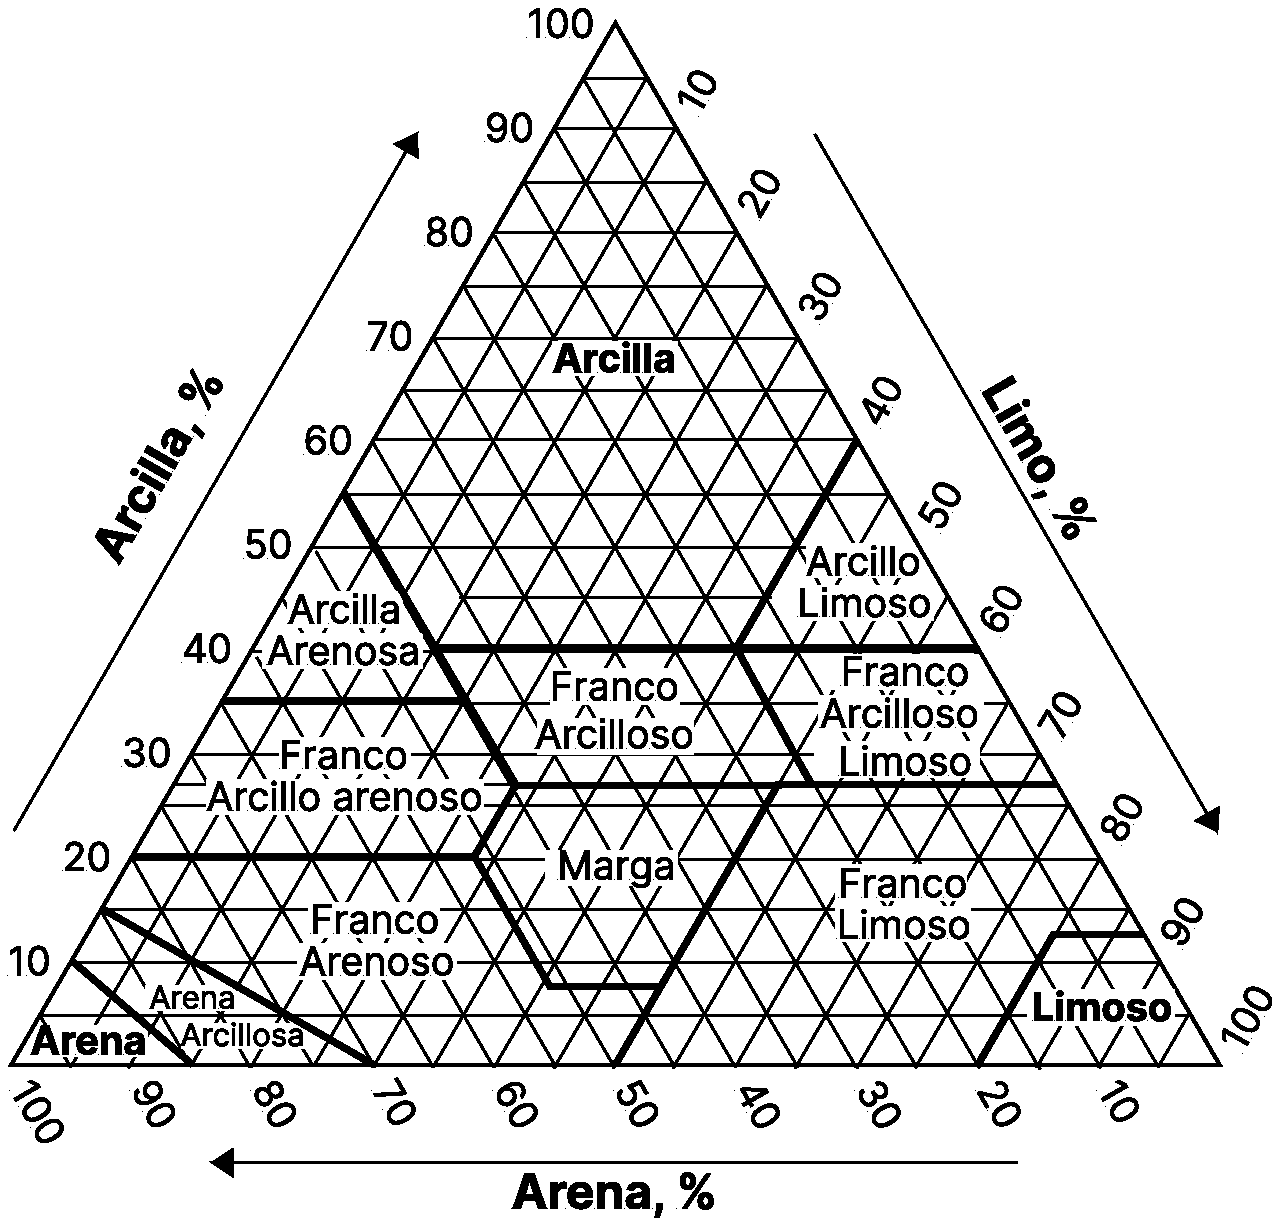
\includegraphics[width=0.8\textwidth]{raspa2.pdf}
  \caption{Triángulo de la Textura del Suelo}
  \label{raspa2}
\end{figure}
Tiene influencia sobre el movimiento del agua en el suelo, la cantidad de agua que puede almacenar un suelo y la facilidad de abastecimiento de nutrientes, agua y aire
\begin{itemize}
    \item Determinación de humedad 
    \item Estimar la lámina aprovechable
    \item Estimación de la capacidad de campo
\end{itemize}
\begin{figure}[h!]
\centering
  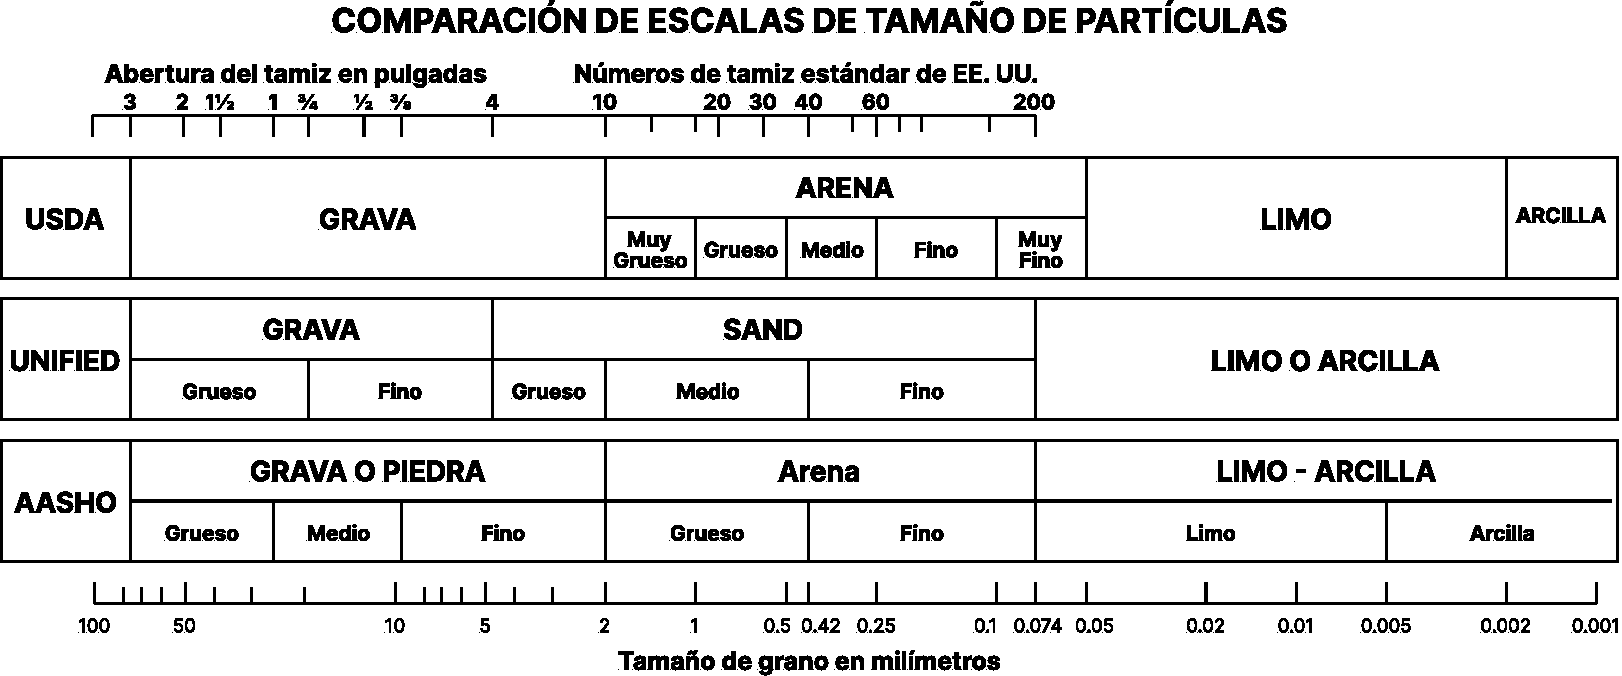
\includegraphics[width=0.8\textwidth]{raspa3.pdf}
  \caption{Granulometría}
  \label{raspa3}
\end{figure}
\subsubsection{Densidad Real}
La densidad se define como la masa por unidad de volumen, constituye la fase sólida del suelo y es un valor poco variable pero en promedio es de $2.65gr/cm^3$

El método más común para la determinación de la densidad real es el de la volumetría, en el cual la determinación del volumen de solidos es factor clave
\begin{equation}
    D_{real} = \frac{M}{V_s}
\end{equation}
\subsubsection{Color del suelo}
Puede identificarse mediante un sistema de color de Munsell, el cuál toma el Matiz, el brillo y el croma\subsection{Características Físicas del Suelo}\subsubsection{Estructura}
\begin{definition}[Agregado]
    Agrupamiento de partículas primarias
\end{definition}
\begin{definition}[Estructura]
    Organización de las arcillas, limo y arcillas para formar agregados del suelo
\end{definition}
Tipos de estructura:
\begin{itemize}
    \item Laminar: Formado por el impacto de gotas, encontradas en horizontes subsuperficiales
    \item Columnar: Bordes redondeados y está en suelos alcalinos
    \item Prismática: En horizontes arcillosos, subsuperficiales y en regiones húmedas
    \item Angular: EN horizontes subsuperficiales
    \item Subangular: Zonas áridas y semiáridas, y pobres en materia orgánica
    \item Granular: La más favorable; son suelos ricos en bases y materia orgánica
    \item Migajosa: En horizontes superficiales de pastizales
\end{itemize}

La clase de los tamaños de los agregados:
\begin{itemize}
    \item Muy fina
    \item Fina
    \item Media
    \item Gruesa
    \item Muy gruesa
\end{itemize}
Sin grado de desarrollo: tiene grano simple: no se forma agregados, granos sueltos, EN horizontes arenosos o muy lixiviados.

Masivos: No se firman agregados ni poros, bloque sin fisuras y en horizontes inferiores

Con grado de desarrollo: 
\begin{itemize}
    \item Débil:Agregados pobres, se deshace y tiene un bajo nivel de organización
    \item Moderado: Agregados bien formados, moderadamente durables y un nivel de organización medio
    \item Fuerte: Agregados buen formado, durables y un nivel de organización alto
\end{itemize}
La estructura del suelo debe ser estable para resistir las fuerzas externas, se realizan labores agrícolas como adherir materia orgánica y no erosión; de 20-30cm granular o migajosa macroporos y en la capa inferior debe tener 30-150 microporos y macroporos

\subsubsection{Densidad aparente}

\begin{definition}[Densidad Aparente]
    Es la masa de suelo por unidad de volumen, es la compactación del suelo, representando la relación entre sólidos y el espacio poroso. Ésta varía con la textura del suelo y el contenido de materia orgánica; puede variar estacionalmente por efecto de labranzas y con la humedad del suelo sobre todo en los suelos con arcillas expandible
\end{definition}
Varía con respecto la textura porque en suelos finos, la Densidad Aparente varía entre 1 y $1.2 g/cm^3$ mientras que en suelos arenosos es mayor y puede variar entre 1.2 y 1.6. La capacidad de almacenamiento de agua, compactación en suelos dedicados a la infraestructura hidroagrícola son de importancia para la ingeniería en Irrigación.

La diferencia entre densidad aparente y real, es que la Densidad Real de las partículas densas del suelo, varía con la proporción de elementos constituyendo el suelo y en general está alrededor de 2.65

\subsubsection{Porosidad}

El espacio poroso del suelo se refiere al porcentaje del volumen del suelo no ocupado por sólidos. Dentro del espacio poroso se puede distinguir los macro y microporos
eq

La clasificación de la porosidad, de acuerdo con sus características de conducción o almacenamiento, puede resumirse en tres categorías:
\begin{enumerate}
    \item Porosidad sub-microscópica
    \item 
\end{enumerate}
La porosidad del suelo superficial se determina:
\begin{itemize}
    \item Procesos de infiltración y escurrimiento del agua
\end{itemize}

\subsubsection{Conductividad Hidráulica}
Describe la capacidad de un suelo para transmitir agua e indirectamente oxígeno hacia el perfil del suelo

En laboratorio, se basa en la toma de muestras en campo, generalmente de forma que conserven su estructura original, lo cual es muy difícil de lograr en la práctica. Se mona  una columna, de forma que las paredes laterales sean impermeables y se pueda hacer circular

\subsubsection{Infiltración}
El proceso de entrada de agua, generalmente vertical, a través de la superficie del suelo, siendo la primera etapa en el movimiento del agua en el suelo.

Dicha entrada tendrá lugar en condiciones no saturadas, sobre todo bajo la influencia de los gradientes de potencial matricial.

\subsubsection{Potencial Hídrico}
Es la magnitud más empleada para expresar y medir el estado de energía libre del agua, es decir la capacidad de sus moléculas para moverse en algún sistema

\subsubsection{Potencial Matricial}
Es la energía del agua debido a la fuerza de retención de los poros y de la adsorción de las partículas del suelo. En suelos saturados su valor es de 0 bar y en insaturados es negativo.

La cantidad de agua aportada por una lluvia o por un riego condiciona el proceso siempre y cuando se cumpla que $P<I$ precipitación< infiltración acumulada (mm)

En aquellos casos en que la intensidad de la lluvia vaya aumentando, llegará un momento donde no pueda infiltrarse
% \subsubsection{Conductividad Térmica}


  \begin{definition}[Materia Orgánica]
    Es el resultado del análisis químico aplicado en el material orgánico midiendo la oxidación de los materiales asociados al carbono, resultando una cantidad de carbono multiplicada por 0.54 (Allan Walkley y Amstrong Black)
  \end{definition}
  \begin{definition}[Material Orgánico]
    Es todo aquello que en su estructura contiene carbono
  \end{definition}
  % La materia orgánica se aplica
  % El nitrógeno en la atmósfera está presente en un 78\%, la cual sirve para enfriar la tierra y no la pueden aprovechar las plantas,

  % % Hacer una tabla de biofertilizantes específico para cada cultivo
  % % nódulos blancos - no activas
  % % nódulos rosas- activas
  % \begin{definition}[Consorcio]
  %   Conjunto de especies para fertilizar
  % \end{definition}refelxión
  % % ¿Existen las vacunas en las plantas?


  % % Alvedo angulo de  del suelo | plasticultura
\subsection{Capacidad de Intercambio Catiónico}
Es el número de sitios de intercambio que existe en el suelo, para la agricultura la montmorillonita (2:1) y la caolinita (1:1), cuando existe el proceso de sustitución isomórfica, hay un desbalance energético (iónico), por lo tanto se perpetua el signo negativo.

Si se tiene un agregado, se alojan un número de sitios que puede contener el suelo, con montmorillonita es mayor, al contrario a la colinita.
\subsection{Potencial Z}
La electronegatividad es una fuerza que es expresada en una partícula, de manera que la potencial Z, es la distancia que tienen los átomos para poder unirse. Esta distancia depende de la arcilla, si es montmorillonita es mayor y en caolinita es menor.
\section{Agua-Suelo}
\subsection{Humedad del agua en el suelo}
Se mide en porcentaje de humedad con respecto el peso de suelo seco, para obtener la cantidad de agua
Supóngase que se tiene un suelo arcilloso o uno arenoso con una capacidad de campo y punto de marchitez permanente,
la diferencia de ambos porcentajes nos da como resultado la Humedad Aprovechable, por lo tanto se recomienda regar al llegar a un
punto entre capacidad de campo y punto de marchitez llamado ``Punto Crítico'' debido al estrés que puede sufrir la planta.
\begin{equation}
    PMP = \frac{1}{2}CC
\end{equation}
La lámina de riego ($L_r$) es calculada con la siguiente fórmula
\begin{equation}
    L_r = \frac{\left(CC - PMP\right) \cdot Da \cdot P_m}{100}
\end{equation}
\subsection{Diseño agronómico de los sistemas de riego}
\subsubsection{Humedad del suelo}
\begin{align}
    &P_s =\frac{P_{sh} - P_{ss}}{P_{ss}} \cdot 100\\
    &P_v =\frac{V_a}{V_t} \cdot 100\\
    &P_v = P_s \cdot Da
\end{align}
Los contenido de agua entre el $P_s$ y la $CC$ es el agua de gravedad; entre el $CC$ y el $PMP$ es la humedad aprovechable agua y debajo del PMP es agua higroscópica, los métodos para determinar o estimar son los siguientes:
\begin{enumerate}
    \item Método gravimétrico
    \item Analizador de humedad (basculas de rayos infrarrojos o halógenos)
    \item Tensiómetro: Sólo sirve cuando hay riego con goteo y mide presión negativa
    \item Bloques de impedancia: El medidor utiliza la resistencia eléctrica para determinar la humedad del suelo. El lector muestra el porcentaje de humedad disponible en el suelo en función de la resistencia eléctrica del mismo.
    \item Aspersor de neutrones: Está cubierta de plomo y elementos radiactivos, es muy preciso pero se requiere capacitación para operarla.
    \item Reflectómetro de dominio de tiempo TDR
    \item Sensores de humedad SM-100 y SM-300
\end{enumerate}

¿Cómo está ubicada el agua en el suelo y fisiológicamente cómo la absorbe la planta?

El agua estructural está en medio de las laminas de los filosilicatos, ni para los procesos biológicos se tomará en cuenta para la clasificación de los tipos de agua para el área agronómica.
% tesis para calibrar el tdr-300, todas las limitaciones arroyo prado yaerli norma.
\begin{definition}[Histeresis]
    Es la tendencia de un material a conservar una de sus propiedades, en ausencia del estímulo que la ha generado
\end{definition}
El agua siempre va a estar absorbida en las paredes de los poros, 

La falta de materia orgánica en suelos arcillosos o suelos limosos (micro poros discontinuos) propicia la formación de microporos

Un suelo tipo Molisol, tiene mesoporos
\subsection{Infiltración}
Es la entrada del agua al suelo, vertical o lateralmente. Cuando se habla de un riego por gravedad
se analiza verticalmente y horizontalmente se estudia para determinar el ancho del surco.
Inclusive cuando son surcos de camas meloneras se interesa el componente horizontal porque el agua
fluye de esa dirección (véase imagen \ref{raspa6})
\begin{figure}[h!]
\centering
  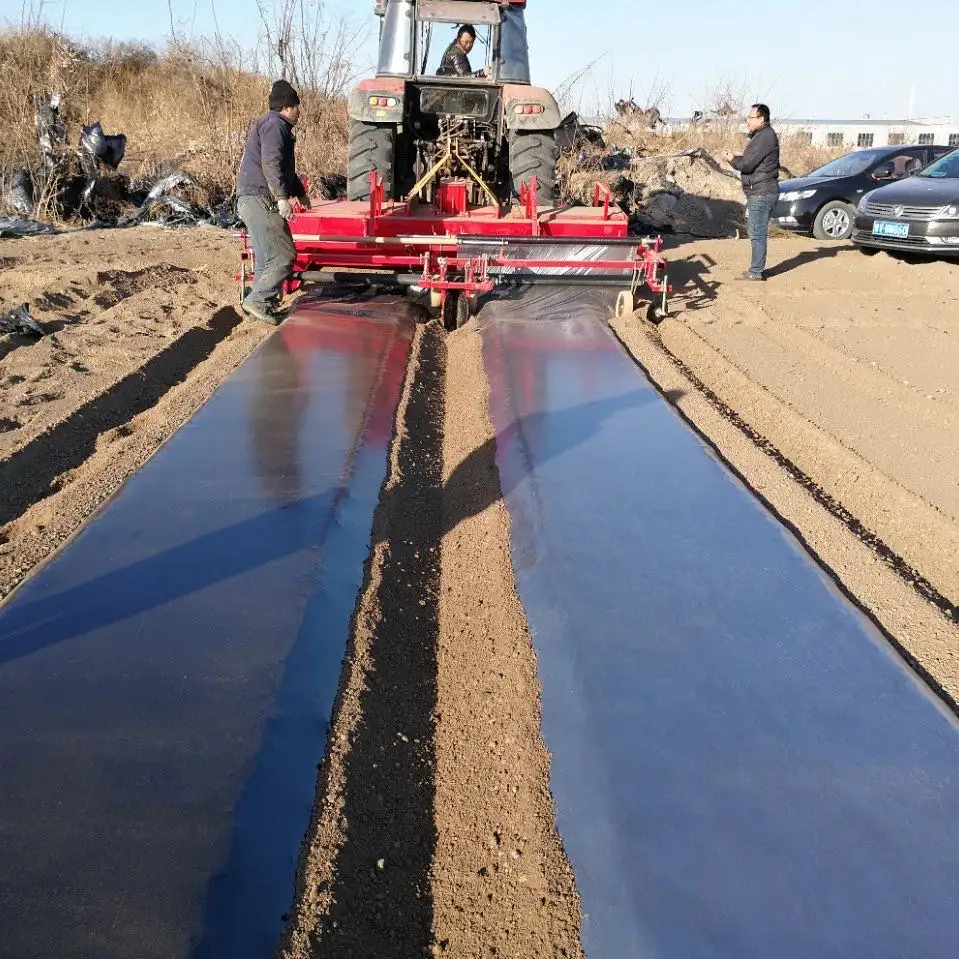
\includegraphics[width=0.5\textwidth]{raspa6.png}
  \caption{Maquinaria agrícola tractor cama shaper ridger, camas elevadas donde la componente de infiltración es horizontal.}
  \label{raspa6}
\end{figure}
\begin{itemize}
    \item Velocidad de infiltración (I en $cm/h$)
    \item Infiltración acumulada o lámina infiltrada, Z
    \item Velocidad de infiltración básica, $I_b$, vease la figura \ref{raspa7}
\end{itemize}
\begin{figure}[h!]
\centering
  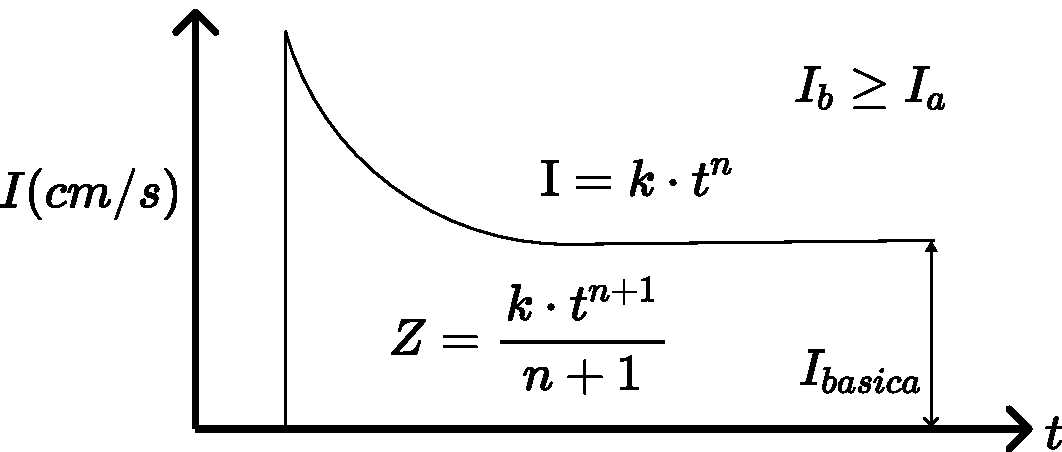
\includegraphics[width=0.5\textwidth]{raspa7.pdf}
  \caption{Componentes de la infiltración ponderando la velocidad de infiltración contra tiempo}
  \label{rapsa7}
\end{figure}
\begin{itemize}
    \item Método del doble cilindro
    \item Método de entradas o salidas
\end{itemize}
Modelo de Kostiakov
\begin{equation}
    I = K\cdot T^n
\end{equation}
\begin{notation}
    \begin{itemize}
        \item $I$ está en cm/h
        \item y $T$ está en minutos
    \end{itemize}
\end{notation}
El volumen acomulado $Z$ usa el factor de conversión de minutos a hora multiplicando por 60 y es la integral de $KT^n$:
\begin{equation}
    Z =\frac{K}{60(n + 2)}\cdot T^{n + 1}
\end{equation}
Modelo del USDA, donde B es la infiltración básica ($B=I_b$):
\begin{equation}
    I KT^n + B
\end{equation}
Por lo tanto la infiltración acomulada es:
\begin{equation}
    Z =\frac{K}{60(n + 1)}\cdot T^{n + 1} + B\cdot T
\end{equation}
Modelo de Philip establece que $n$ prácticamente es $1/2$, por lo tanto:
\begin{equation}
    Z = S\cdot T^{\frac{1}{2}}+ b\cdot T
\end{equation}
Lo que la infiltración sería:
\begin{equation}
    \frac{dZ}{dT} =\frac{S}{2\cdot T} + b
\end{equation}
\subsection{Eficiencia de riego}
\begin{equation}
    E = E_c \cdot E_a \cdot 100
\end{equation}
Eficiencia de aplicación:
\begin{equation}
    E_a = \frac{V_r}{V_t} \cdot 100
\end{equation}
\begin{figure}[h!]
\centering
  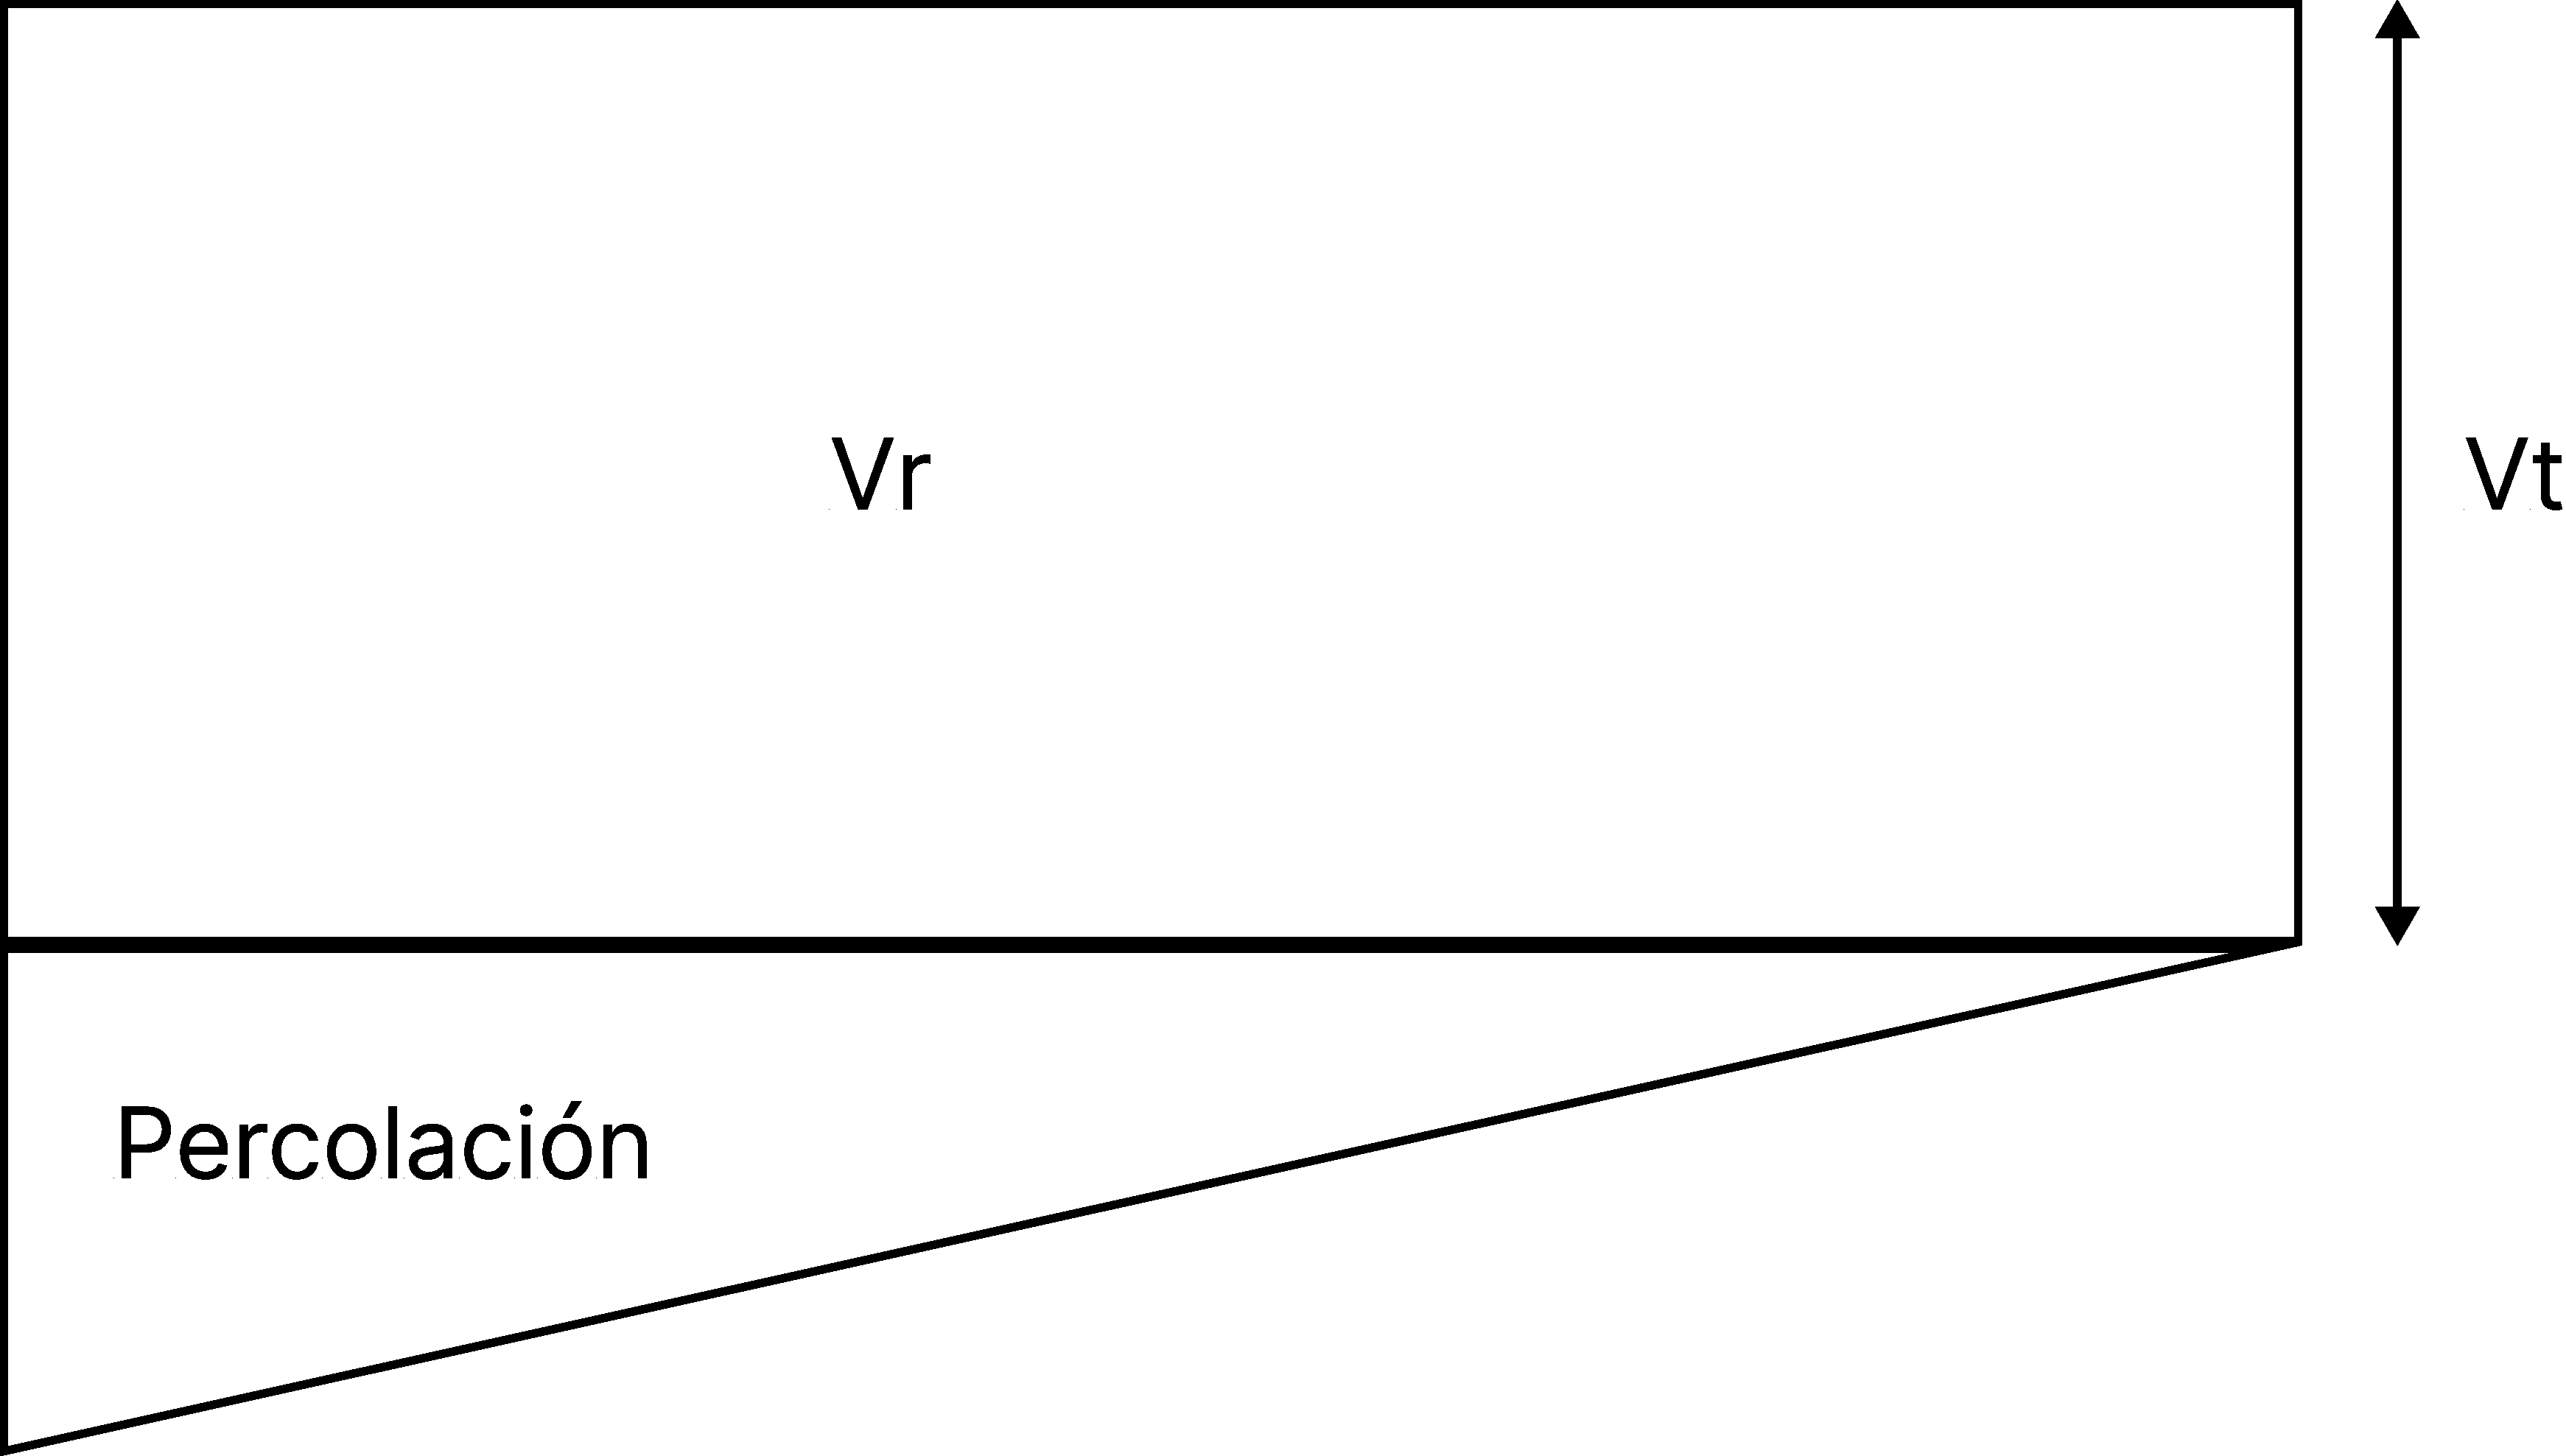
\includegraphics[width=0.5\textwidth]{raspa4.pdf}
  \caption{Eficiencia de aplicación}
  \label{raspa4}
\end{figure}
Eficiencia de requerimiento o almacenamiento $E_r$
\begin{equation}
    E_r = \frac{V_t}{V_r} \cdot 100
\end{equation}
\begin{figure}[h!]
\centering
  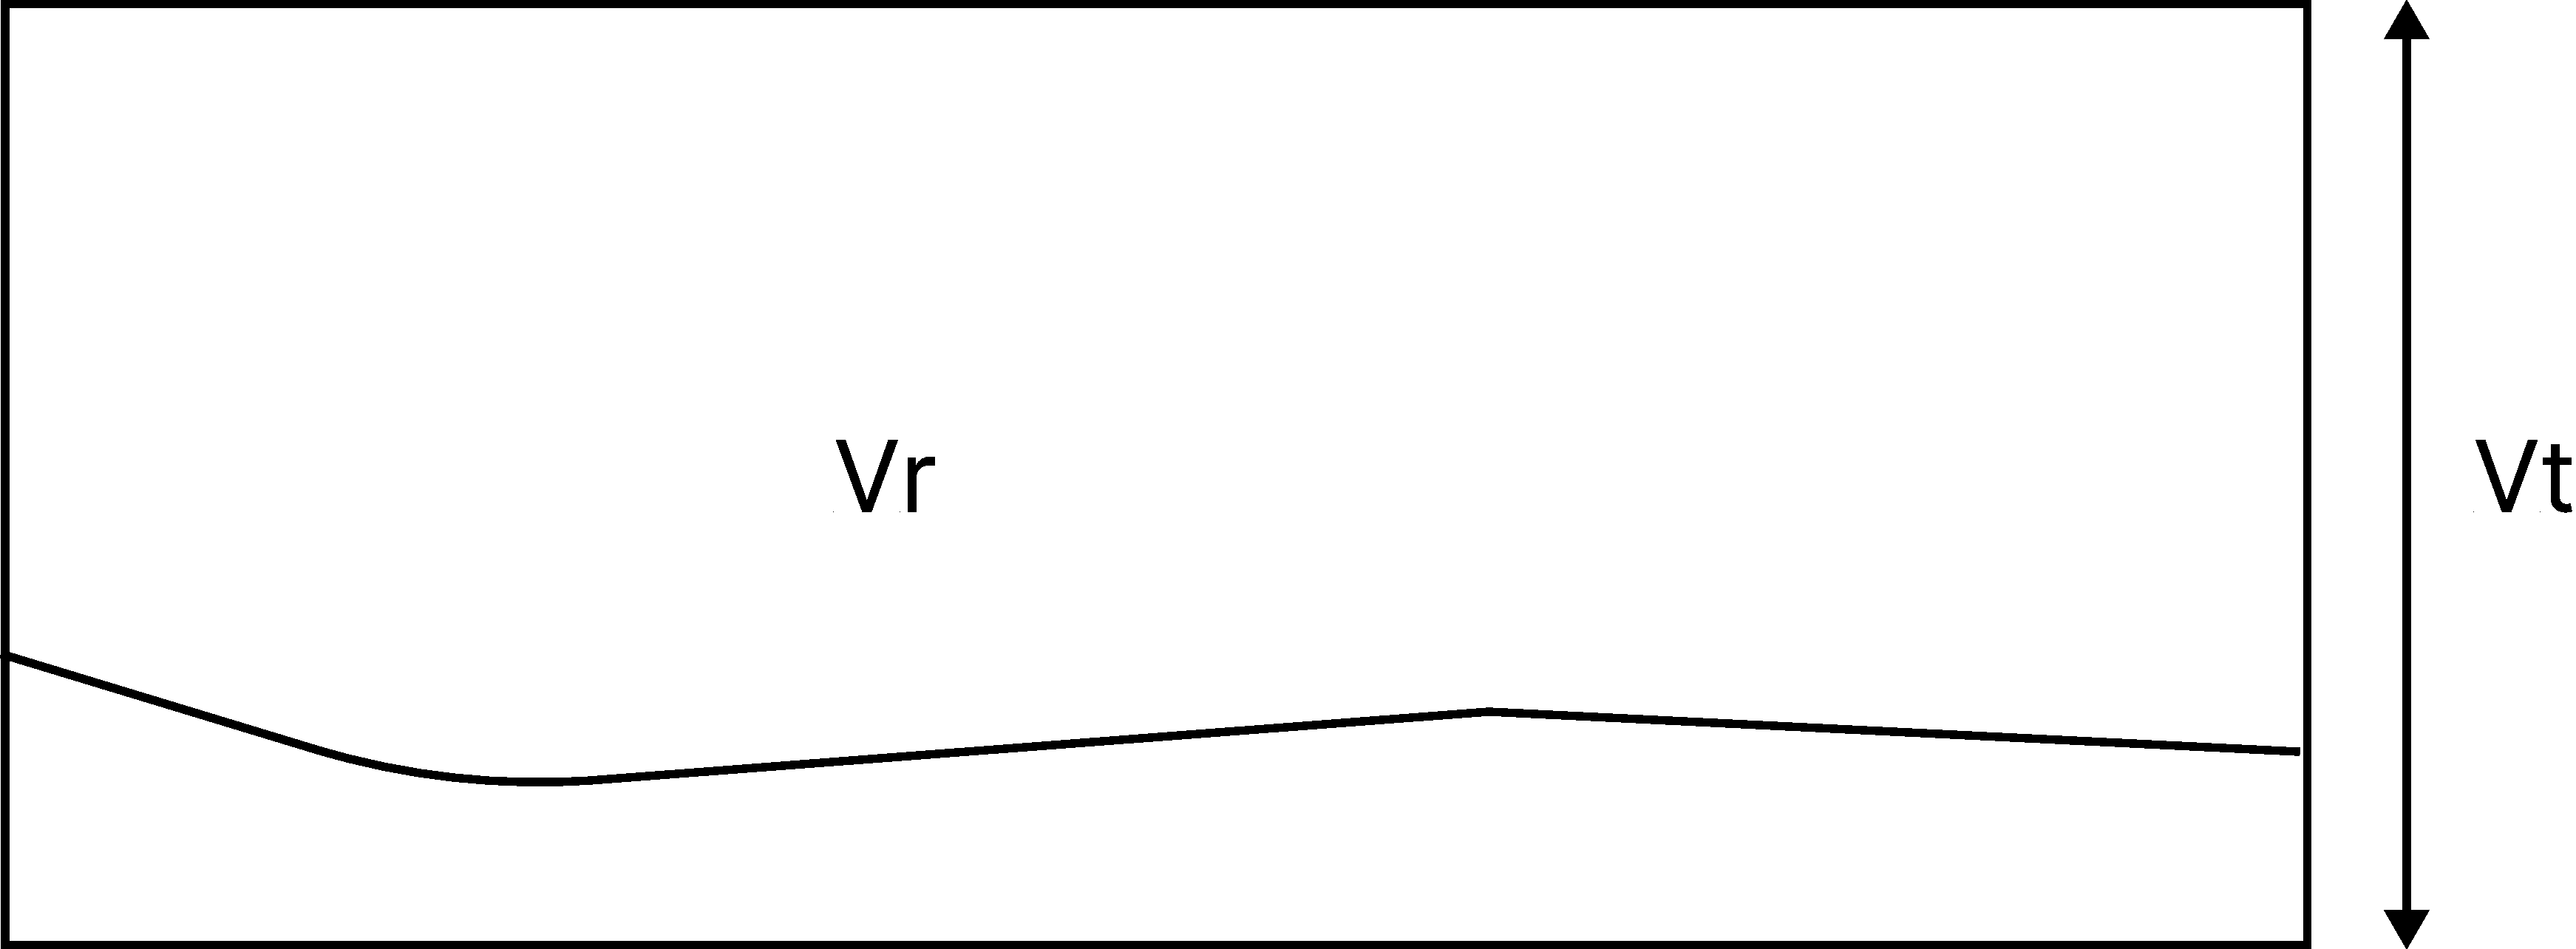
\includegraphics[width=0.5\textwidth]{raspa5.pdf}
  \caption{Eficiencia de almacenamiento, ni siquiera hubo pérdidas de percolación}
  \label{raspa5}
\end{figure}
% Cuando tiene una eficiencia de aplicación, que tenga un valor menor al 100\% significa que se tiene un volumen de percolación. Por lo tanto la eficiencia de requerimiento es mayor al 100\%. Cuando la eficiencia de aplicación es mayor al 100\%
Eficiencia de distribución o coeficiente de uniformidad
\begin{equation}
    E_d = CU =\left(1 -\frac{\sum\left\lvert L_i -\bar{L}\right\rvert}{n\bar{L}}\right) \cdot 100
\end{equation}
\section{Sistema Planta}
Los cloroplastos están conformados en su núcelo con magnecio, puesto que éste es el único elemento que posee un radio hidráulico hidratado que alcanza la exitación para romper los enlaces que existen entre el $CO_2$ el magencio genera esa vibración, como luz de onda fotosintética, haciendo que los demás compuestos se estructuran formando bloques de carbohidráto.

Se dice que alrededor de 250 factores interactúan con la planta y es necesario depurar cuáles son aquellos que se involucran en la hidratación del cultivo (priorización).

Tan sólo la planta necesita el 1\% para cumplir todas sus necesidades básicas, sin embargo el resto 

Cómo es que el agua consume agua líquida y evapotranspira vapor de agua, tiene un cambio brusco de temperatura, rompiendo los enlaces del puente de hidrógeno.
\subsection{Inflitración}
La infiltración, en riego, se considera como la entrada vertical del agua en el suelo. Conocer éste fenómeno es importante porque permite tener un criterio para definir si un riego se está aplicado adecuadamente o no. Otra aplicación importante es determinar el tiempo de riego, es decir, el tiempo que debe estar en contacto el agua con el suelo para aplicar una lámina de riego deseada.

Hay varias maneras de expresar la infiltración, tales como:
\begin{itemize}
    \item Velocidad de Infiltración (I). Es la relación entre la lámina que se infiltra y el tiempo
    que tarda en hacerlo, cm/h o cm/min (L/T).
    \item Infiltración acumulada (Z). Es la integración de la velocidad de infiltración, en
    unidades de lámina (L).
    \item Velocidad de Infiltración básica (Ib). Es la velocidad de infiltración constante, que se
    obtiene después de un determinado tiempo.
\end{itemize}


% Todas las raíces tienen la misma estructura fisiológica, más la membrana
% que ha desarrollado la planta mediante la evolución, varia mucho de especia a especie.

% Las plantas necesitan estar en un porcentaje de saturación del 100\%, luego hay un equilibrio de difusión dependiendo la humedad relativa.

% Las raíces son las únicas estructuras que permiten exudar o extraer los nutrientes, 

% Debe evitarse usar las fichas técnicas, pues aunque dan orientación del ambiente, o los suelos de origen,
% podemos entender la estructura del cultivo está adaptado a ese ambiente y no necesariamente
% implica que forzosamente deben de sembrarse en ese tipo de suelo o clima.

Potencial hídrico: predecir cuál será la ruta que tomará el agua, el suelo en contiene una solución de agua, en el ambiente, en la planta, etc. Por lo tanto el agua siempre va hacia donde hay menos concentración; \textbf{Difusión} De mayor a menor concentración y la \textbf{Homeostasis}

Si hay una Membrana semipermeable es un proceso osmótico, de otra manera es difusión, y en el sistema debe indicarse a qué dirección va

En conclusión el potencial hídrico funciona por la difusión para \textbf{moverse}.
\begin{equation}
    \Psi= \Psi_0 + \Psi_S + \Psi_{\rho} + \Psi_g + \Psi_m + \Psi_v
\end{equation}
\begin{definition}[Potencial Hídrico]
    Es la energía potencial que posee una masa de agua. Depende de una serie de factores: \textbf{Planta}: dependen de su ecofisiología; \textbf{Concentración} ($\Psi_S$, potencial osmótico): El agua fluirá desde una solución poco concentrada hasta una solución más concentrada tomando en cuenta la planta y los electrolitos o sales en el sistema suelo. - \textbf{Presión} ($\Psi_{\rho}$, turgencia): El agua fluirá desde un sistema con presión alta hasta un sistema con baja presión. - \textbf{Altura} ($\Psi_g$, potencial gravitacional): El agua fluirá hacia abajo. - \textbf{Suelo} ($\Psi_m$, potencial matricial): Proviene de todos los procesos de adsorción y desorción del suelo,  Mezcla de $\Psi_S$ y $\Psi_{\rho}$ este potencial se origina por las fuerzas de capilaridad y tensión superficial en espacios pequeños. - \textbf{Humedad} ($\Psi_v$, presión de vapor): Es el mismo término que la turgencia, pero es más correcto emplear este para la medición de potenciales en el vapor de agua. - \textbf{Carga eléctrica} ($\Psi_c$, potencial eléctrico): El agua no tiene carga, lo ignoraremos. - \textbf{De referencia} ($\Psi_0$): Es el potencial hídrico que posee el agua pura en condiciones estándar de temperatura y presión. Es muy difícil establecer un valor concreto, por convenio se le ha asignado el valor 0.
\end{definition}
\subsubsection{Ecofisiología}
Las plantas nos permiten modificar el entorno, cómo se cuantifica de la interrelación de los cuatro sistemas: agua-suelo-planta-atmósfera es a través del potencial hídrico que describe adónde va el agua.

Existen modelos matemáticos ``predictivos'' (menor variables con la menor dispersión); y ``teóricos'' (mayor variables que explican el fenómeno)

Casi siempre se mide la presión, la lógica para usar éste potencial es saber para dónde se mueve el agua, evidentemente el cómo se mueve definirá ésta interrogante:
\begin{itemize}
    \item En un modelo predictivo, se solicita la temperatura, el cultivo, tipo de suelo, humedad relativa, presión atmosférica, precipitación, velocidad del viento, radiación, etc.
    \item Para el potencial atmosférico: se necesita temperatura, y humedad relativa
    \item Para el potencial Osmótico: se necesita la conductividad eléctrica  
    \item Potencial gravitacional: Velocidad de infiltración, puesto que indirectamente nos menciona las propiedades físicas de poros, estructura, textura y materia orgánica
    \item Potencial  matricial: Textura, capacidad de almacenamiento del agua que depende claramente de las propiedades físico químicas del suelo de potencial z y capacidad de intercambio catiónico, similar a la capacidad de campo, con la distinción que no necesariamente tiene que dejar de drenar por 24 horas. Sin los instrumentos puede deducirse el tipo de arcilla a partir del intemperismo
    \item Potencial planta: Tipo del cultivo
\end{itemize}
\subsection{Cálculo de la Eto}
\subsubsection{Precipitación efectiva}
\begin{align*}
    &Pe = Cp \cdot P
    &Cp = \frac{\frac{E}{P}}{1.53 + 0.8\left(\frac{Et}{P}\right)}
\end{align*}
El otro método del Servicio de Conservación de Suelos del USDA es:
\begin{align*}
    &Pe = P \cdot \left(1 -\left(\frac{0.2 \cdot P}{125}\right) \right)\quad \text{Cuando P} \leq \frac{250mm}{periodo}\\
    &Pe = 125 +(0.1 \cdot P)\quad \text{Cuando P} > \frac{250mm}{periodo}
\end{align*}
\begin{figure}[h!]
\centering
  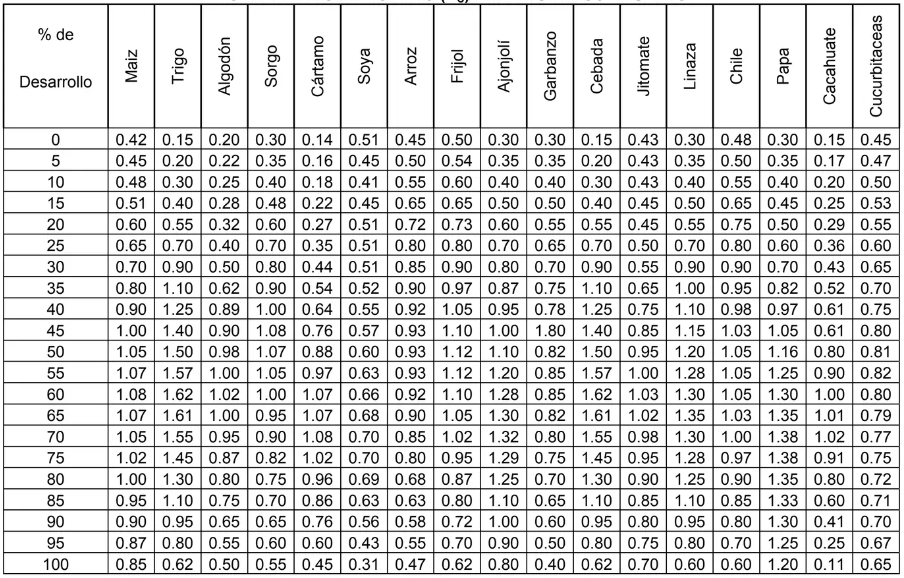
\includegraphics[width=0.5\textwidth]{raspa8.png}
  \caption{Tablas para calcular los coeficientes de cultivo}
  \label{raspa8}
\end{figure}
\begin{figure}[h!]
\centering
  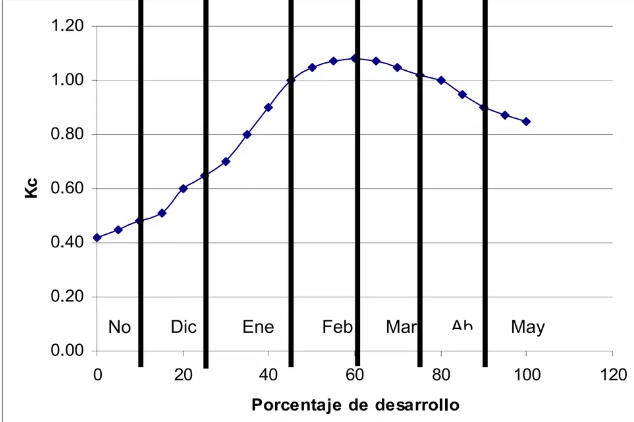
\includegraphics[width=0.5\textwidth]{raspa9.png}
  \caption{Curva para calcular los coeficientes de cultivo gráficamente}
  \label{raspa9}
\end{figure}
Existen cuatro fases de desarrollo
\begin{itemize}
    \item Fase inicial
    \item Fase de desarrollo del cultivo
    \item Fase de mediados del período
    \item Fase final
\end{itemize}
\begin{figure}[h!]
\centering
  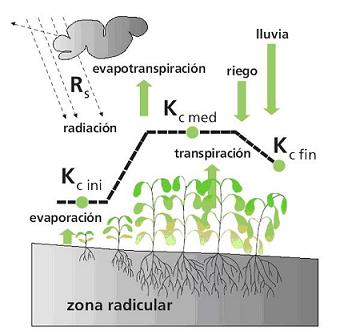
\includegraphics[width=0.5\textwidth]{raspa10.jpg}
  \caption{Curva de coeficiente del cultivo}
  \label{raspa10}
\end{figure}
\section{Programa de riego}
Tipos de calendarización de riegos:
\begin{enumerate}
    \item Basados en el balance de humedad del suelo
    \item Monitoreo del suelo
    \item Monitoreo del cultivo
\end{enumerate}

\subsection{Método analítico}

Balance de agua en el suelo:
\begin{equation}
    HA_i = HA_{i + 1} + P_i + R_i + ET_i + PP_i
\end{equation}
\begin{notation}Donde todas las unidades están en mm:
    \begin{itemize} 
        \item $HA_i$ Humedad almacenada en día i
        \item $HA_{i-1}$ Humedad almacenada en día anterior
        \item $P_i$ Precipitación ocurrida en día 
        \item $R_i$ Riego de día i
        \item $ET_i$ Evapotranspiración en día
        \item $PP_i$ Percolación profunda en día
    \end{itemize}
\end{notation}
% Condiciones del balance, en la ecuación anterior se considera que hay deficiencia cuando:
% \begin{equation}
%     HA_{i - 1} + P_1 - ET_i < 0
% \end{equation}






% Textura
% Se refiere a la proporción relativa de arena, limo y arcilla del suelo. La importancia de su estudio radica en la influencia que este tiene en la cantidad de agua que puede almacenar un suelo; el movimiento del agua en el suelo: la facilidad de abastecimiento de nutrientes, de agua y de aure, de gran importancia para la vida de las plantas. Los límites de tamaño (arena limo y arcilla), de acuerdo con las clasificaciones americana e internacional, aparecen en el cuadro:
% (...img)
% Para representarlas se puede utilizar la clasificación del Departamento de agricultura de los Estados Unidos, según el triángulo de texturas mostrado en la figura, en el qué se toman en consideración los porcentajes de arcillas, limos y arenas.
% (...img)
% En términos generales, los suelos se dividen en suelos de textura fina y suelos de textura gruesa.

% En los suelos de textura fina predomina la arcilla y tienen una mayor capacidad de adsorción de nutrientes, usualmente son más fértiles. Los suelos arenosos tienen poros grandes y permiten una más rápida infiltración del agua. Sin embargo, los suelos arcillosos tienen una mayor capacidad de retención de agua debido a  su mayor área superficial; tienen un volumen de vacíos total mayor qué los suelos arenosos.
% Estructura
% Desde el punto de vista morfológico, el término estructura del suelo se ha definido cómo la disposición o arreglo de las partículas primarias (arcilla, limo, arena) la capacidad estructural del suelo se define cómo su capacidad de formar peds espontáneamente y de qué estos Peds se dividan en pedazos pequeños, granos o agregados, sin la intervención del hombre.
% Aunque hay muchas clases de agregados reconocidos en la morfología del suelo, el granular es el más importante en la producción de cultivos; ésta estructura granular es la que se considera cómo la más conveniente.
% La estructura afecta la penetración del agua, el drenaje, la aireación y el desarrollo de raíces, afectando así la productividad del suelo y las facilidades de labranza. Especialmente en el suelo superficial, puede ser alterada por las labores de cultivo, mientras qué la textura no cambia por las operaciones usuales de labores.
% (...img)
% Granular: Relativamente no poroso; agregados pequeños (tamaño menor de 2cm de diámetro), esferoides, no ajustados a los agregados adyacentes. Se localizan comúnmente en el horizonte A
% Migajosa: Relativamente porosos; agregados pequeños y esferoidales no ajustados
% Laminar: Agregados similares a placas; las dimensiones verticales de los agregados posición natural son menores qué sus dimensiones horizontales. Las placas a menudo se sobreponen e impiden la permeabilidad. Se encuentran generalmente en el horizonte A2, en suelos de bosque y estratos arcilloso
% Bloques: Bloques limitados por otros agregados, citas caras angulares bien definidas, forman el molde de estos. Los agregados a menudo se rompen en bloques más pequeños. Se localizan generalmente en el horizonte B
% Bloques Subangulares: Gránulo similares a bloques limitados por otros agregados, cuyas caras angulares redondeadas forman el molde del gránulo. Se localiza generalmente en el horizonte B
% Prismática: Agregados similares a columnas con las partes superiores no redondeadas. Otros agregados forman el molde del ped. Algunos agregados prismáticos se rompen en peds de bloques más pequeños. Se localizan generalmente en el horizonte B
% Columnar: Se caracteriza porque las dimensiones verticales de los agregados en posición natural son mayores qué sus dimensiones horizontales. Las columnas están separadas por grietas verticales y generalmente quebradas por grietas horizontales. Las cabezas de las columnas son redondeadas y se encuentran muy a menudo en el horizonte B, en suelos sódicos.
% Densidad aparente
% Es el cociente qué resulta de dividir el peso de suelo seco entre el volumen total, incluyendo los poros. Usualmente se expresa en gr/cm3. Para fines prácticos, conceptualmente esto es lo mismo qué la gravedad específica o peso volumétrico.
% \begin{equation}
% Da=\frac{Pss}{Vt}
% \end{equation}
% Los suelos arenosos son relativamente bajos en espacio vacío total y proporcionalmente tienen densidades aparentes altas.
% Las densidades aparentes aumentan con la profundidad en el perfil del suelo. Esto se debe a más bajos niveles de materia orgánica, menor agregación y más compactación.
% Los valores de la densidad aparente varían en función de las propuedades de los suelos fundamentalmente con la textura y el contenido de materia orgánica. Sin embargo cómo valores medios se tienen los siguientes:
% \begin{table}[h!]
% \centering
% \begin{tabular}{@{}cc@{}}
% \toprule
% Textura          & Densidad Aparente   \\ \midrule
% Arenas           & $1.6-1.7\,gr/cm^3$  \\
% Francos          & $1.3-1.4\,gr/cm^3$  \\
% Arcillas         & $1.0-1.2\,gr/cm^3$  \\
% Suelos orgánicos & $0.7-1.0\, gr/cm^3$ \\ \bottomrule
% \end{tabular}
% \caption{Valores medios de la densidad aparente}
% \label{tab}
% \end{table}
% Densidad real
% La densidad real de un suelo, es la relación que existe entre el peso de pestem en seco (Pss) y el volumen real o sea el volumen de sus partículas (VP), usualmente se expresa en $gr/cm^3$
% \begin{equation}
% Dr=\frac{Pss}{Vp}
% \end{equation}
% El tamaño y arreglo de las partículas del suelo no afectan la densidad de las partículas. Sin embargo, la materia orgánica qué pesa mucho menos de un volumen de sólidos minerales influirá en ella. En suelos minerales está densidad es caso constante y varía de $2.6-2.75gr/cm^3$.
% Porosidad
% El espacio poroso es la porción de suelo no ocupado por partículas sólidas, los espacios porosos están ocupados por aire y agua. El arreglo de las partículas sólidas del sueli determinan la cantidad de espacio poroso.

% La porosidad se define cómo el porcentaje de volumen total de suelo qué está ocupado por los poros:
% \begin{equation}
% Pr=\frac{V}{Vt}\times 100
% \end{equation} 
% Área específica
% La superficie específica es una propiedad de los sólidos la cual es la relación entre el área superficial total y la masa del sólido,o volumen en bruto,​ o área en la sección transversal.

% Es una magnitud científica derivada que puede ser utilizada para determinar el tipo y propiedades de un material (por ejemplo tierra). Se la define tanto como área superficial dividida por masa (en cuyo caso sus unidades son $m2/kg$), o área superficial dividida por el volumen (en cuyo caso sus unidades son a$ m^2/m^3$ o $m^{-1}$).

% Es una magnitud que posee especial importancia en el caso de análisis de adsorción, catálisis heterogénea, y reacciones en superficies.






























































































